Lors de ce projet proposé par Coveo \href{https://www.coveo.com/fr}{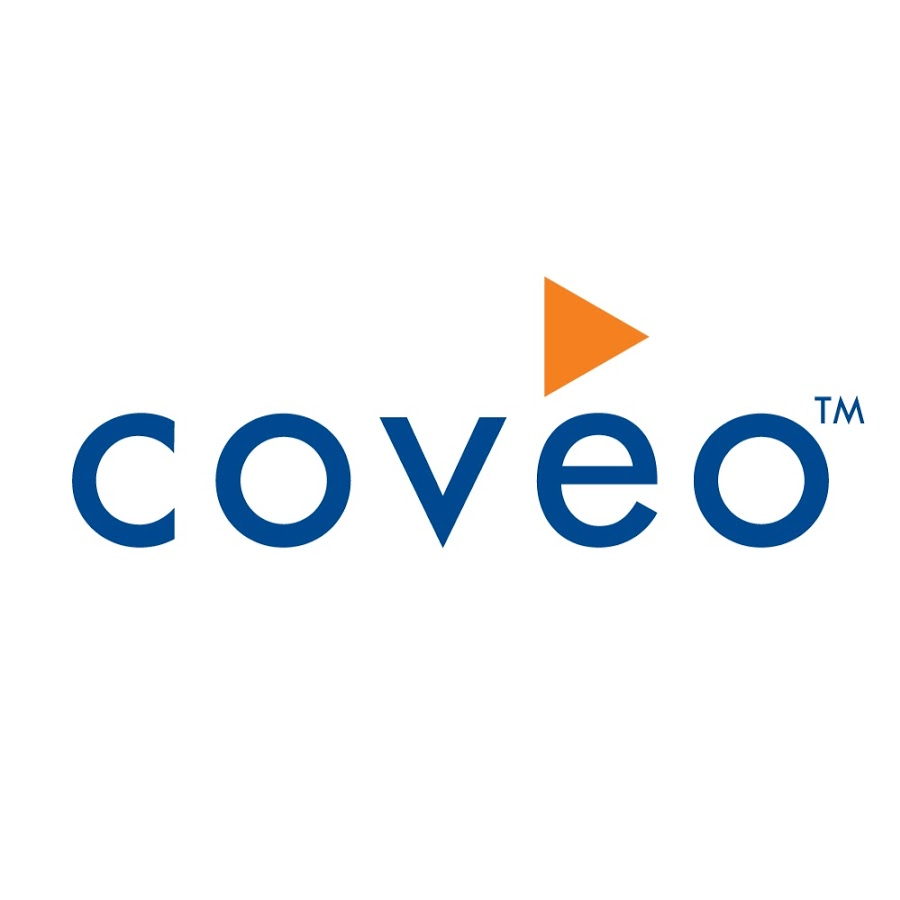
\includegraphics[height=0.3cm]{coveo_logo}}, nous devions utiliser un historique de requêtes faites par des utilisateurs afin de développer un modèle de recommandation de document. 
Le but du modèle est de proposer une série de 5 documents d'intérêt en fonction de la recherche qui est faite par l'utilisateur et de certaines autres caractéristiques.

Toutefois, dans la plupart des approches les plus populaires, (METTRE DES RÉFÉRENCES DE PAPIERS QUI PARLENT DE TECHNIQUES) le modèle commence par extraire de l'information des documents cible et peut par la suite se définir une mesure de distance entre une requête et chacun des documents pour déterminer quel serait la meilleure correspondance requête-document. 
Malheureusement, pour ce projet, nous n'avons pas accès au contenu des documents que l'on souhaite prédire, mais bien à un jeu restreint de caractéristiques telles la source du document, son auteur et son titre.

